\section{Einführung - 3.10.2012}

Numerische Mathematik befasst sich mit der näherungsweisen Lösung von Problemstellungen (mit dem Computer).
%\begin{itemize}
  %\item Formulierung
  %\item Entwicklung
  %\item Untersuchung
  %\item Implementierung
    %von Verfahren und Algorithmen
%\end{itemize}
\begin{equation*} 
  \left.
  \begin{aligned} 
   & \text{Formulierung} \\ 
   & \text{Entwicklung} \\ 
	 & \text{Untersuchung} \\
 	 & \text{Implementierung} \\
  \end{aligned} 
  \right\} 
  \text{von Verfahren und Algorithmen} 
\end{equation*} 
Von der Problemstellung zur Näherungslösung:

  \begin{empheq}{alignat*=3} 
   & \text{physikalisches, chemisches, ... Problem bzw. Modell} & \smarttag{Modellfehler} \\ 
   & \text{mathematisches Modell (z.B. DGL)} & \smarttag{Diskretisierungsfehler} \\ 
	 & \text{numerisches Näherungsverfahren (endlich} & \Smarttag{Verfahrensfehler}\\
	 & \text{ dim. Ersatzproblem)} \\
 	 & \text{Algorithmen für Ersatzprobleme} & \smarttag{Impl.-fehler z.B. Rundungsfehler}\\
	 & \text{Implementierung} & \\
  \end{empheq}
Die letzten drei Punkte werden von der Numerik abgedeckt.\\
\textbf{ZIEL}: (möglichst) genau, möglichst schnell, mit möglichst geringem Aufwand (z.B. Speicher)

\subsection{Gleitpunktzahlen $\Fhat$}
\begin{align*}
		\Fhat = \F \cup \F_d \hspace{0.5cm} \text{mit} \hspace{0.5cm} & \F && \text{normalisierte Gleitpunktzahlen}\\
		 &\F_d && \text{denormalisierte Gleitpunktzahlen} 
\end{align*}
\para{Normalisierte GPZ}

\begin{align*}
x = \sigma\,\cdot\,M\,\cdot\,\,b^e \hspace{0.5cm} \text{mit} \hspace{0.5cm} & \sigma && \text{Vorzeichen}\\
& M && \text{Mantisse} \\
& b && \text{Basis} \\
& e && \text{Exponent}
\end{align*}

\begin{align*}
M = \sum^t_{k=1} d_k b^{-k} \hspace{0.5cm} \text{mit} \hspace{0.5cm} & d_1,\ldots,d_t\, \in\,\{0,1,\ldots,b-1\} && \text{Ziffern der Mantisse}\\
& t && \text{Mantissenlänge} \\
& d_1 \neq 0 && \text{(Normalisierung)} \\
& e_{min} \leq e \leq e_{max} && \text{Exponentenbereich}
\end{align*}

Schreibweise:
\begin{equation*}
x = \sigma\,(0.d_1d_2d_3\,\ldots\,d_t)b^e
\end{equation*}

\para{Denormalisierte GPZen}
\begin{figure}[htbp]
  \centering
  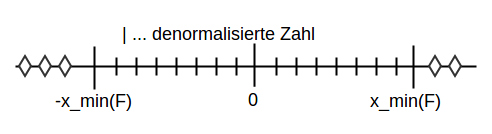
\includegraphics[width=0.7\textwidth]{figures/denormalisiertezahlen.png}
  \caption{Zahlenstrahl mit denormalisierten und normalisierten Zahlen}
  \label{fig:denormalisiert}
\end{figure}

\begin{align*}
x_d = \sigma\,M\,b^{e_{min}} &\\
M = \sum^t_{k=2} d_k b^{-k} \hspace{0.5cm} \text{mit} \hspace{0.5cm} & d_2,\ldots,d_t\, \in\,\{0,1,\ldots,b-1\} \\
& \text{keine Normierung} 
\end{align*}

\para{Gleitpunktzahlsystem}
\Fhatfunc{b,t,$e_{min}$,$e_{max}$}

\example{Beispiel: "`Doppeltes Grundformat"' ("`double"' in C, Java, MATLAB)}

\Fhatfunc{2,\,53,\,-1021,\,1024} Im PC als 64bit $\rightarrow$ 52 + 1 da erstes bit ungleich 0 sein muss, 11 Stellen für Exponenten / Umschaltung zu denorm. GPZ. Symbolische Ausdrücke ("`Inf"',"'NaN"',...) 
kleinste/größte pos Zahl:
\begin{align*}
	& x_{min}(\F) =  2^{-1022}\,\approx\, 2,23\cdot\,10^{-308} \\
	& x_{max}(\F) \approx 1,8\,\cdot\,10^{308} \\
  & x_{min}(\Fhat) \approx 5\cdot\,10^{-324} & \text{nicht in diesen Bereich gehen!}
\end{align*}

\subsubsection{Rundung}
Die Abbildung $\mathrm{rd}: \mathbb{R} \rightarrow \Fhat, x\,\mapsto\,\mathrm{rd}(x)$ heißt Rundung, wenn $|\mathrm{rd}(x)-x|=min|y-x|, y\in\,\F$. 
\todo{realtiver Fehler unterbringen}
\begin{empheq}[innerbox=\fbox,right=\Leftarrow{\text{gilt nur für normalisierte Zahlen}}]{align*}
\text{Für} \hspace{1cm} x_{min}(\F)&\leq\,|x|\,\leq\,x_{max}\,(\F) \hspace{1cm}\text{gilt:}\\
\frac{|rd(x)-x|}{x}&\leq \frac{1}{2}\,b^{-t+1} \eqqcolon eps \leftarrow \text{Maschinengenauigkeit}
\end{empheq}

Es sei $\frac{\mathrm{rd}(x)-x}{x}=\delta\,\Rightarrow\,\mathrm{rd}(x)=x(1+\delta)$
es gilt:
\begin{empheq}[innerbox=\fbox]{align*}
  \mathrm{rd}(x)=x(1+\delta) & \hspace{1cm} |\delta|\leq\,eps
\end{empheq}

\example{Maschinengenauigkeit für "`double"'}
\Fhatfunc{2,\,53,\,-1021,\,1024}
\begin{equation*}
eps = \frac{1}{2}\,2^{-53+1}\approx\,1,1\cdot\,10^{-16}
\end{equation*}
Maschinenepsilon 
\begin{equation*}
\epsilon_M=2 eps = b^{-t+1}
\end{equation*}

$\epsilon_M$ ist der Abstand zwischen 1 und der nächstgrößeren GPZ.

\subsubsection{Gleitpunktarithmetik}
Schon elementare Operationen von GPZen führen zu Resultaten, die nicht im $\Fhat$
liegen, zB $\frac{1}{3} \not \in \Fhat$. \\
Maschinenoperationen: $\oplus$, $\ominus$, $\odot$, $\oslash$ \\
Genaue Operation: $\Box$ \\
Standard für die Genauigkeit von Maschinenoperationen (IEEE 754): \\

\begin{empheq}[innerbox=\fbox]{align*}
  x \circ y &= \mathrm{rd}(x \Box y)   \\ 
\text{für} \hspace{0.5cm} x, y \in \Fhat, x_{min}(\F) &\leq | x \circ y | \leq x_{max}(\F)\\
  & \Updownarrow \\
 x \circ y & = (x \Box y)(1 + \delta) \hspace{0.5cm} \text{mit} \hspace{0.5cm} |\delta | \leq eps
\end{empheq}

\subsubsection{Fehlerverstärkung bei elementaren Rechenoperationen}
Fragestellung: Wie wirken sich fehlerbehaftete Eingangsdaten bei elementaren
Rechenoperationen aus? Kann es zu einer wesentlichen Fehlerverstärkung kommen?
Ja, es kommt aber darauf an.
\example{Bsp:}
$ f(x)=\frac{1 - \cos(x)}{x^2} $ für $x=1.2 \cdot 10^{-5} $
Angenommen wir runden $\cos(x)$ auf 10 Stellen genau \\
\begin{align*}
 \cos(x) &\approx 0.999 999 999 9 =: c \\
 \frac{1 - c}{x^2} &= \frac{10^{-10}}{1.44 \cdot 10^{-10}} = 0.6944\dots 
\end{align*}
Mit Hilfe der Taylorreihe lässt sich zeigen, dass $ f(x) \in [0, \frac{1}{2}) $. \\
relativer Fehler $ \geq \frac{0.69 - 0.5}{0.5} = 38\% $ \\

\para{Fehlerverstärkung bei Addition (Subtraktion)}
Seien $ a, b \in \mathbb{R} $ gegeben und
$ \tilde{a} = \mathrm{rd}(a) = a (1 + \delta_{a}) $ mit $ | \delta_{a} | \leq eps $ sowie
$ \tilde{b} = \mathrm{rd}(b) = b (1 + \delta_{b}) $ mit $ | \delta_{b} | \leq eps $ \\
Relative Fehler\\
\begin{equation*}
\left| \frac{\tilde{a} + \tilde{b} - (a + b)}{a + b} \right| =
\left| \frac{a\delta_{a} + b\delta_{b}}{a + b} \right| \leq eps \frac{|a| + |b|}{|a + b|} 
\end{equation*}
Ist $ |a + b| \ll |a| + |b| $ dann kann der relative Fehler groß werden.
D.h. bei der Subtraktion zweier annähernd gleich großer Zahlen, können
sich Eingangsfehler erheblich verstärken. $\Rightarrow$ \large{\textcolor{rot}{\textbf{AUSLÖSCHUNG
signifikanter Stellen}}}

\para{Fehlerverstärkung bei Multiplikation}
Seien $ a, b \in \mathbb{R}\setminus\{0\} $ gegeben und
$ \tilde{a} = \mathrm{rd}(a) = \frac{a}{1 + \delta_{a}} $ mit $ | \delta_{a} | \leq eps $ sowie
$ \tilde{b} = \mathrm{rd}(b) = \frac{b}{1 + \delta_{b}} $ mit $ | \delta_{b} | \leq eps $ \\
Relative Fehler
\begin{gather*}
\left| \frac{\tilde{a}\tilde{b} - a b}{a b} \right| =
\left| \frac{\frac{ab}{(1 + \delta_{a})(1 + \delta_{b})} - ab}{ab}\right| = \\
\left| \frac{ab - ab(1 + \delta_{a})(1 + \delta_{b})}{ab(1 + \delta_{a})(1 + \delta_{b})} \right| =
\left| \frac{ab(\delta_{a} + \delta_{b} + \delta_{a}\delta_{b})}{ab(1 + \delta_{a})(1 + \delta_{b})} \right| \leq
\frac{3eps}{1 - 3eps} \leq 4eps 
\end{gather*}
$\Rightarrow$ Multiplikation führt nicht zu einer wesentlichen Fehlerverstärkung.
Dasselbe lässt sich auch für die Division zeigen.

\subsection{Landau-Symbole (``$\LandauO$-Notation'')}
Verwendung zur:
\begin{itemize}
  \item Beschreibung des asymptotischen Verhaltens von Funktionen
  \item Effizienzverhalten von Algorithmen
\end{itemize}
Definition: Seien $f,g: \mathbb{R} \to \mathbb{R}$
\begin{enumerate}[(a)]
  \item $f(x) = \LandauO(g(x))$ für $x \to a :\Leftrightarrow$
    Es gilt $c > 0$ und $\delta > 0$, so dass für alle $x \in \{|y - a| < \delta\}: |f(x)| \leq c|g(x)| \Leftrightarrow$ in etwa ähnliches Verhalten
  \item $f(x) = \LandauO(g(x))$ für $x \to \infty :\Leftrightarrow$
    Es gilt $c > 0$ und ein $x_0 > 0$, so dass für alle $x > x_0:\,|f(x)| \leq c|g(x)| \Leftrightarrow$ $f(x)$ wächst nicht schneller als $g(x)$
  \item $f(x) = o(g(x))$ für $x \to \Box \in \mathbb{R} \cup \{\pm \infty\} :\Leftrightarrow
    \underset{x \to \Box}{\lim}|\frac{f(x)}{g(x)}| = 0$
\end{enumerate}

\example{Beispiel:}
\begin{align*}
  \frac{x + 1}{x^2} &= \LandauO(\frac{1}{x}) \text{ für } x \to \infty \text{ , denn } \\
  \frac{1}{x} + \frac{1}{x^2} &\leq \frac{1}{x} + \frac{1}{x} = \underbrace{2}_c \frac{1}{x} \text{ für } x \geq \underbrace{1}_{x_0}
\end{align*}
\begin{align*}
  x^{\alpha} = o(x^{\alpha + 1}) \text{ für } x \to \infty \text{ , denn }
  \frac{x^{\alpha}}{x^{\alpha + 1}} = \frac{1}{x} \xrightarrow[x\to\,\infty]{}0
\end{align*}
\textcolor{rot}{VORSICHT}: Das Gleichheitszeichen ist bei Verwendung der Landau-Symbole rein symbolisch
zu verstehen: Symmetrie $[a = b \Leftrightarrow b = a]$ und Transitivität 
$[a = b \wedge b = c \Rightarrow a = c]$ gelten i.A. nicht. \\
z.B.: $x = \LandauO(x^2)$ für $x \to \infty$ aber $x^2 \neq \LandauO(x)$ für $x \to \infty$

\subsection{Fehleranalyse}
Bei der Analyse der Fehlerfortpflanzung bei der Lösung von mathematischen Problemen
unterscheidet man:
\begin{itemize}
  \item Kondition des Problems
  \item Stabilität des Algorithmus (zur Lösung des Problems)
\end{itemize}
\para{Kondition eines Problems}
Mathemathisches Problem sei durch eine Funktion beschrieben: $H:X \to Y$ \\ 
$\underbrace{x}_{\textrm{Input}} \mapsto \underbrace{H(x)}_{\textrm{Resultat}}$\\
Fehlberbehafteter Input $x + \Delta x$ mit $\Delta x$ als Fehler
\begin{align*}
  \frac{|| H(x + \Delta x) - H(x)||}{|| H(x) ||} = ?
\end{align*}
\para{Satz von Taylor (Taylorreihenentwicklung):}
\begin{enumerate}[(a)]
  \item Sei $f: I \in \mathbb{R} \to \mathbb{R}\,$ (n + 1)-mal stetig differenzierbar, dann gilt für
    $x, \Delta x \in I$: \\
    $f(x + \Delta x) = f(x) + \Delta x f^{\prime}(x) + 
    \frac{(\Delta x)^2}{2!}f^{\prime\prime}(x) + \ldots + 
    \frac{(\Delta x)^n}{n!}f^n(x)+
    \frac{(\Delta x)^{n + 1}}{(n + 1)!}f^{n + 1}(\zeta(x)) $ \\
    wobei $x \leq \zeta(x)\leq x + \Delta x$
  \item Sei $f: \mathbb{R}^n \to \mathbb{R}^m\,$ 2 mal stetig differenzierbar \\
    $f(x + \Delta x) = f(x) + \Delta x f^{\prime} + R(x, \Delta x) $ \\
    wobei $||R(x, \Delta x)|| = \LandauO(||\Delta x||^2)$ für $||\Delta\,x|| \to 0$
\end{enumerate}

\para{Absoluter Fehler:}
$\Delta H(x) := H(x + \Delta x) - H(x)$ wenn $||\Delta x|| \ll 1$ ist, dann \\
$\Delta H(x) \cong H^{\prime} \Delta x$

\para{Relative Fehler (1D Fall):}
\begin{align*}
  \delta H(x) := \frac{\Delta H(x)}{H(x)} \mathrel{\widetilde{=}} 
  \frac{H^{\prime} \Delta x}{H(x)} =
  \frac{x H^{\prime}(x)}{H(x)} \cdot \frac{\Delta x}{x}
\end{align*}
Verstärkerfunktion $=: \kappa(H, x) = | \frac{x H^{\prime}(x)}{H(x)} |$ \\
relative Eingangsfehler $:= \delta x = \frac{\Delta x}{x}$
\begin{empheq}[innerbox=\fbox]{align*}
  |\delta H(x)|  \cong \kappa(H, x) |\delta x|
\end{empheq}
$\kappa(H, x)$ wird (relative) Kondition(szahl) des Problems $H$ für den Input $x$
genannt. (Mehrdimensionaler Fall: Analoge Definition; verwende Normen statt Beträge) \\
Ein Problem heißt \underline{gut konditioniert}, falls die Konditionszahl klein (nahe bei 1) ist
(für die infragekommenden Inputs).

\example{Beispiel:}
Die Nullstellen der quadratischen Gleichung $\lambda^2 - 2x\lambda + 1 = 0$ sind für $x > 1$ gegeben durch 
$\lambda_1 = x +\sqrt{x^2 - 1} \;\;\; \lambda_2 = x - \sqrt{x^2 - 1}$ \\
Konditionszahl für $\lambda_2 = H(x)$
\begin{align*}
  \kappa(H, x) = \left|\frac{x H^{\prime}(x)}{H(x)}\right| = 
  \left|\frac{x[1 - \frac{1}{2}(x^2 - 1)^{-\frac{1}{2}} 2x]}{x - \sqrt{x^2 - 1}} \right| =
  \left|\frac{\frac{x(\sqrt{x^2 - 1} - x)}{\sqrt{x^2 - 1}}}{x - \sqrt{x^2 - 1}}\right| =
  \left|- \frac{x}{\sqrt{x^2 - 1}}\right|
\end{align*}
Fallunterscheidung:
\begin{enumerate}[(i)]
  \item $x \gg 1:\ \kappa(H, x) \approx 1 \Rightarrow$ gut konditioniert
  \item $x \approx 1:\ \kappa(H, x)$ groß $\Rightarrow$ schlecht konditioniert
\end{enumerate}
Berechnung der Lösung für i)
\begin{enumerate}[(a)]
  \item $H(x) = x - \sqrt{x^2 - 1}$ numerisch instabil (Auslöschung)
  \item $H(x) = \frac{(x - \sqrt{x^2 - 1})(x + \sqrt{x^2 - 1})}{x + \sqrt{x^2 - 1}} = $
    $\frac{1}{x + \sqrt{x^2 - 1}}$ numerisch stabil
\end{enumerate}

\para{Stabilität eines Algorithmus}
Dafür gibt es verschiedene uneinheitliche Konzepte und Definitionen. \\
\underline{Komperative Erklärung}: \\
Algorithmus I zur Lösung eines Problemes ist stabiler als Algorithmus II,
wenn der Gesamteinfluss der Rundungsfehler bei Algorithmus I kleiner als
bei Algorithmus II ist.

